\documentclass{article}
\usepackage{amssymb}
\usepackage{amsfonts}
\usepackage{amsmath}
\usepackage{graphicx}
\usepackage{minted}

\author{Jonathan Kalsky}
\date{March 26 2026}
\title{\normalsize CSCE 222\\ \Large Homework 4}
\linespread{1.5}

\begin{document}
\maketitle
\tableofcontents
\vspace{1cm}

\section[3.2]{Exercises for Section 3.2}

\subsection[14]{Question 14 - Determine whether $x^3$ is O(g(x)) for each of these functions g(x).}

\subsubsection[a]{(a) g(x)=$x^2$}
If C and k are witnesses, the inequality $x^3 \leq C(x^2)$ holds for all x $>$ k\\
$x^3 \leq C(x^2)$ $\equiv$ $x \leq C$ | Division by $x^2$\\
However, no matter what C and k are, x is arbitrarily large will not be bounded by a constant. \\Since the inequality does not hold for a pair of witnesses C and k, this contradiction shows that $x^3$ is not O($x^2$)

\subsubsection[b]{(b) g(x)=$x^3$}
\textbf{Definition: }$f(x) \; is \;O(g(x)) \Longleftrightarrow if \; |f(x)| \leq C|g(X)|$ for all x$>k$ where C$>$0\\
\textbf{Proof:}\\
$f(x) = |x^3| = x^3$\\
$x^3 \leq C|x^3| = Cx^3$\\
Let C = 1 and k = 0\\
$x^3 \leq x^3$ which is true for all x $>$ 0\\
Since witnesses exist for this relationship, it is true that f(x) is bounded by g(x) for some constant C if $x>k$. Therefore $x^3$ is O(g(x)).

\subsubsection[c]{(c) g(x)=$x^2 + x^3$}
\textbf{Definition: }$f(x) \; is \;O(g(x)) \Longleftrightarrow if \; |f(x)| \leq C|g(X)|$ for all x$>k$ where C$>$0\\
\textbf{Proof:}\\
$f(x) = |x^3| = x^3$\\
$x^3 \leq C|x^3 + x^2| = Cx^3 + Cx^2$\\
Equivalent to $1\leq C + \frac{C}{x}$ by dividing both sides by $x^3$\\
Let C = 1 and k = 0\\
$1 \leq 1 + \frac{1}{x}$ which is true for all x $>$ 0\\
Since witnesses exist for this relationship, it is true that f(x) is bounded by g(x) for some constant C if $x>k$. Therefore $x^3$ is O(g(x)).

\subsubsection[d]{(d) g(x)=$x^2 + x^4$}
\textbf{Definition: }$f(x) \; is \;O(g(x)) \Longleftrightarrow if \; |f(x)| \leq C|g(X)|$ for all x$>k$ where C$>$0\\
\textbf{Proof:}\\
$f(x) = |x^3| = x^3$\\
$x^3 \leq C|x^4 + x^2| = Cx^4 + Cx^2$\\
Equivalent to $1\leq Cx + \frac{C}{x}$ by dividing both sides by $x^3$\\
Let C = 1 and k = 1\\
$1 \leq x + \frac{1}{x}$ which is true for all x $>$ 1\\
Since witnesses exist for this relationship, it is true that f(x) is bounded by g(x) for some constant C if $x>k$. Therefore $x^3$ is O(g(x)).

\subsubsection[e]{(e) g(x)=$3^x$}
\textbf{Definition: }$f(x) \; is \;O(g(x)) \Longleftrightarrow if \; |f(x)| \leq C|g(X)|$ for all x$>k$ where C$>$0\\
\textbf{Proof:}\\
$f(x) = |x^3| = x^3$\\
$x^3 \leq C|3^x| = C3^x$\\
Equivalent to $3log_3x \leq xlog_3(3) + log_3(C)$ \\
Equivalent to $3log_3x \leq x + log_3(C)$\\
Let C = 1 and k = 10\\
$3log_3x \leq x $ which is true for all x $>$ 10\\
Since witnesses exist for this relationship, it is true that f(x) is bounded by g(x) for some constant C if $x>k$. Therefore $x^3$ is O(g(x)).

\subsubsection[f]{(f) g(x)=$x^3/2$}
\textbf{Definition: }$f(x) \; is \;O(g(x)) \Longleftrightarrow if \; |f(x)| \leq C|g(X)|$ for all x$>k$ where C$>$0\\
\textbf{Proof:}\\
$f(x) = |x^3| = x^3$\\
$x^3 \leq C|x^3/2| = \frac{C}{2}x^3$\\
Equivalent to $1\leq \frac{C}{2}$ by dividing both sides by $x^3$\\
Let C = 2 and k = 0\\
$1 \leq 1$ which is true for all x $>$ 0\\
Since witnesses exist for this relationship, it is true that f(x) is bounded by g(x) for some constant C if $x>k$. Therefore $x^3$ is O(g(x)).

\subsection[18]{Question 18 - Let k be a positive integer. Show that $1^k + 2^k + \cdots + n^k$ is $O(n^{k+1})$}
\textbf{Definition: }$f(x) \; is \;O(g(x)) \Longleftrightarrow if \; |f(x)| \leq C|g(X)|$ for all x$>l$ where C$>$0\\
\textbf{Proof:}\\
$f(x) = 1^k + 2^k + \cdots + n^k$\\
\indent \indent $\leq n^k + n^k + \cdots + n^k$\\
\indent \indent $= n(n^k) = n^{k+1} = g(x)$\\
since f(x) $\leq n^{k+1}$ as long as x $>$ 0 \\
l = 0 and C = 1 exist for the big O relationship, therefore $1^k + 2^k + \cdots + n^k$ is $O(n^{k+1})$. Escentially since each terms base is n instead of (n-i) for any integer i $<$ n+1, g(x) is always greater than or equal to f(x) 

\subsection[22]{Question 22 - Arrange the functions $(1.5)^n, n^{100}, (logn)^3
, \sqrt{n} logn, 10^n, (n!)^2, n^{99} +n^{98}$ in a list so that each function
is big-O of the next function. }

$(logn)^3 , \sqrt{n} logn , n^{99}+n^{98}, n^{100}, 1.5^n , 10^n, (n!)^2 $

\subsection[26]{Question 26 - Give a big-O estimate for each of these functions. For the function g in your estimate f (x) is O(g(x)), use a simple function g of smallest order.}
\subsubsection[a]{$(n^3 +n^2 logn)(logn+1) +(17 logn+19)(n^3 +2)$}
$f(x) = (n^3 +n^2 logn)(logn+1) +(17 logn+19)(n^3 +2)$\\
\textbf{Theorem 1:} $f_1(x) \; is \; O(g_1(x))\; and \; f_2(x)\; is \; O(g_2(x)) \Longrightarrow (f_1f_2)(x) \; is\; O(g_1(x)g_2(x))$\\
\textbf{Theorem 2:} $f_1(x) \; is \; O(g_1(x))\; and \; f_2(x)\; is \; O(g_2(x)) \Longrightarrow (f_1+f_2)(x) \; is\; O(g(x))$, where $g(x) = max(|g_1(x)|,|g_2(x)|)$ for all x.\\
\vspace{0.5cm}

\noindent First, the product of $(n^3 +n^2 logn)(logn+1)$ will be estimated\\
$(n^3 +n^2 logn) \leq Cn^3 = g(x)$\\
Let C = 2: $(1 + \frac{logn}{n}) \leq 2$ for all x$>$0\\
$(logn +1) \leq Clogn =g(x)$\\
Let C = 2: $(logn +1) \leq 2logn$ for all x $>$ 10\\
By Theorem 1, the product is $O(n^3logn)$\\\vspace{0.5cm}

\noindent Next the product of $(17 logn+19)(n^3 +2)$ will be estimated\\
$(17 logn+19) \leq Clogn = g(x)$\\
Let C = 36: $(17 logn+19) \leq 36logn$\\ for all x$>$10\\
$(n^3 +2) \leq Cn^3 = g(x)$\\
Let C = 3: $(n^3 +2) \leq 3n^3$ for all x>1\\
By Theorem 1, the product is $O(n^3logn)$\\\vspace{0.5cm}

\noindent By theorem 2: $g(x) = max(|g_1(x)|,|g_2(x)|) = max(n^3logn, n^3logn) = n^3logn$\\
Therefore, Our estimate is $O(n^3logn)$

\subsubsection[b]{$(2^n +n^2)(n^3 +3^n)$}
\textit{Note(further correction):} the problem only asks to give a big o estimate and not to provide a comprehensive proof\vspace{0.5cm}

\noindent
$f(x) = (2^n +n^2)(n^3 +3^n)$\\
By combining our functions the greatest term will be the product and sum of the greatest terms:\\
The fastest growing term is: $(2^n)(3^n) = 2^n3^n = 6^n = g(x)$\\
Therefore $O(g(x)) = C(a^n)$ for all n $>$ k and some constant a\\
Our estimate is $O(a^n)$

\subsubsection[c]{$(n^n +n2^n +5^n)(n!+5^n)$}
$f(x) = (n^n +n2^n +5^n)(n!+5^n)$
By combining our functions the greatest term will be the product and sum of the greatest terms:\\
The fastest growing term is: $g(x) = (n^n)(n!) = n!n^n$\\
Therefore $O(g(x)) = C(n!n^n)$ for all n $>$ k\\
Our estimate is $O(n!n^n)$

\section[3.3]{Exercises for Section 3.3}
\subsection[2]{Question 2 - Give a big-O estimate for the number additions used in
this segment of an algorithm.}

\begin{minted}[linenos]{text}
    t := 0
    for i := 1 to n
    for j := 1 to n
    t := t +i +j
\end{minted}
The outer loop runs n times computing n addition\\
The inner loops runs n times for every outer loop, computing $n^2$ additions\\
There are $n^2$ iterations of line 4, where there are 2 additions, computing $2n^2$ additions.\\
Estimating the big O estimate for the number of additions:\\
$n + 3n^2 \leq Cn^2 = g(x)$, Let C = 4, $3n^2 + n \leq 4n^2$ for all x$>$1. The algorithm is $O(n^2)$

\subsection[4]{Question 4 - Give a big-O estimate for the number of operations, where an operation is an addition or a multiplication, used in this segment of an algorithm (ignoring comparisons used to test the conditions in the while loop).}

\begin{minted}[linenos]{text}
    i := 1
    t := 0
    while i <= n
    t := t +i
    i := 2i
\end{minted}
The loop runs for n times but gets cut shorter by a factor due to the doubling of i each iteration.\\
at the end the term of i is = $2^k$ where k is how many times it looped.\\
$2^k = n \Longrightarrow k = log_2 n$\\
Ignoring comparisons, the total additions or substractions occur inside the loop.
Line 4 has 1 addition, and Line 5 has 1 multiplication.\\
$(1+1)log_2n \leq Clogn = g(x)$, Let C = 10, $2log_2n \leq 10logn$ for all x$>$1\\
Due to this shortcut in approaching n, the estimate is $O(logn)$

\pagebreak

\section[Ex.1]{Exercises 1}
\begin{figure}[h!]
    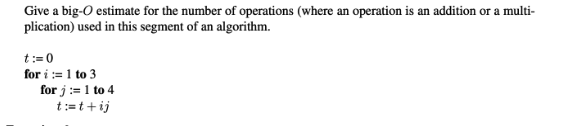
\includegraphics{EX1.png}
\end{figure}

\noindent The outer loop runs 2 time, computing 2 additions\\
The inner loop runs 3 times twice, computing 6 additions\\
Inside the inner loop there is 1 addition, and 1 multiplication\\
These are the only multiplication/addition operations\\
$2+6+6(2) \leq C(1) = g(x)$\\
Let C = 21, $20 \leq 21$ for all x $>$ 0\\
Therefore, the big O estimate for this algorithm segment is $O(1)$

\section[Ex.2]{Exercises 2}
\begin{figure}[h!]
    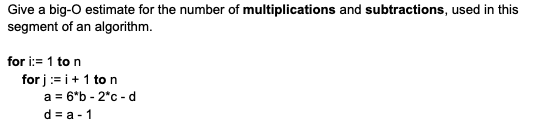
\includegraphics{EX2.png}
\end{figure}
\noindent The outer loop runs n times, computing n additions\\
The inner loop runs $\frac{n}{2}$ times n-1 times, computing $\frac{n^2 - n}{2}$ additions\\
Setting a takes 2 multiplications and 2 subtractions\\
Setting d takes 1 subtraction\\
$\frac{n^2 - n}{2} + n$ $+ (2+2+1)\frac{n^2 - n}{2} \leq Cn^2 = g(x)$\\
Let C = 3, $3n^2 -2n \leq 3n^2$ for all x $>$ 0\\
Therefore, the big O estimate for this algorithm segment is $O(n^2)$


\end{document}